\documentclass[11pt,a4paper]{article}
\usepackage[utf8]{inputenc}
\usepackage[T1]{fontenc}
\usepackage{lmodern}
\usepackage[margin=2cm]{geometry}
\usepackage{graphicx}
\usepackage{xcolor}
\usepackage{hyperref}
\usepackage{enumitem}
\usepackage{titlesec}
\usepackage{parskip}
\usepackage{needspace}
\usepackage{ifthen}
\raggedbottom

% Define colors
\definecolor{darkgray}{HTML}{333333}
\definecolor{gray}{HTML}{666666}
\definecolor{lightgray}{HTML}{999999}

% Hyperlink setup
\hypersetup{
    colorlinks=true,
    linkcolor=darkgray,
    urlcolor=darkgray,
}

% Section formatting
\titleformat{\section}{\Large\bfseries\color{darkgray}}{}{0em}{}[\titlerule]
\titleformat{\subsection}{\large\bfseries\color{darkgray}}{}{0em}{}
\titlespacing*{\section}{0pt}{20pt}{10pt}
\titlespacing*{\subsection}{0pt}{15pt}{5pt}

% Custom commands
\newcommand{\cvitem}[2]{\textbf{#1}: #2}
\newcommand{\cventry}[5]{%
    \ifthenelse{\equal{#1}{Elvia – Unified Messaging Platform (Convey)} \OR \equal{#1}{Norwegian Police IT – UTSYS}}%
        {\needspace{12\baselineskip}}%
        {\needspace{10\baselineskip}}%
    \noindent\textbf{#1} \hfill \textcolor{gray}{#2}\\
    \textit{#3}\\
    #5
    \vspace{0.5em}
}

% Remove page numbers
\pagestyle{empty}

\begin{document}

% Header with photo
\begin{minipage}[t]{0.7\textwidth}
\vspace{0pt}
{\Huge\bfseries Christopher H\ae rem}\\[5pt]
{\Large Senior Full-Stack Engineer | Tech Lead \& Consultant}\\[10pt]
Oslo, Norway\\
\href{mailto:chris.haerem@gmail.com}{chris.haerem@gmail.com}\\
\href{https://github.com/CHaerem}{GitHub: CHaerem} \quad
\href{https://linkedin.com/in/chaerem}{LinkedIn: chaerem}
\end{minipage}
\begin{minipage}[t]{0.3\textwidth}
\vspace{0pt}
\raggedleft
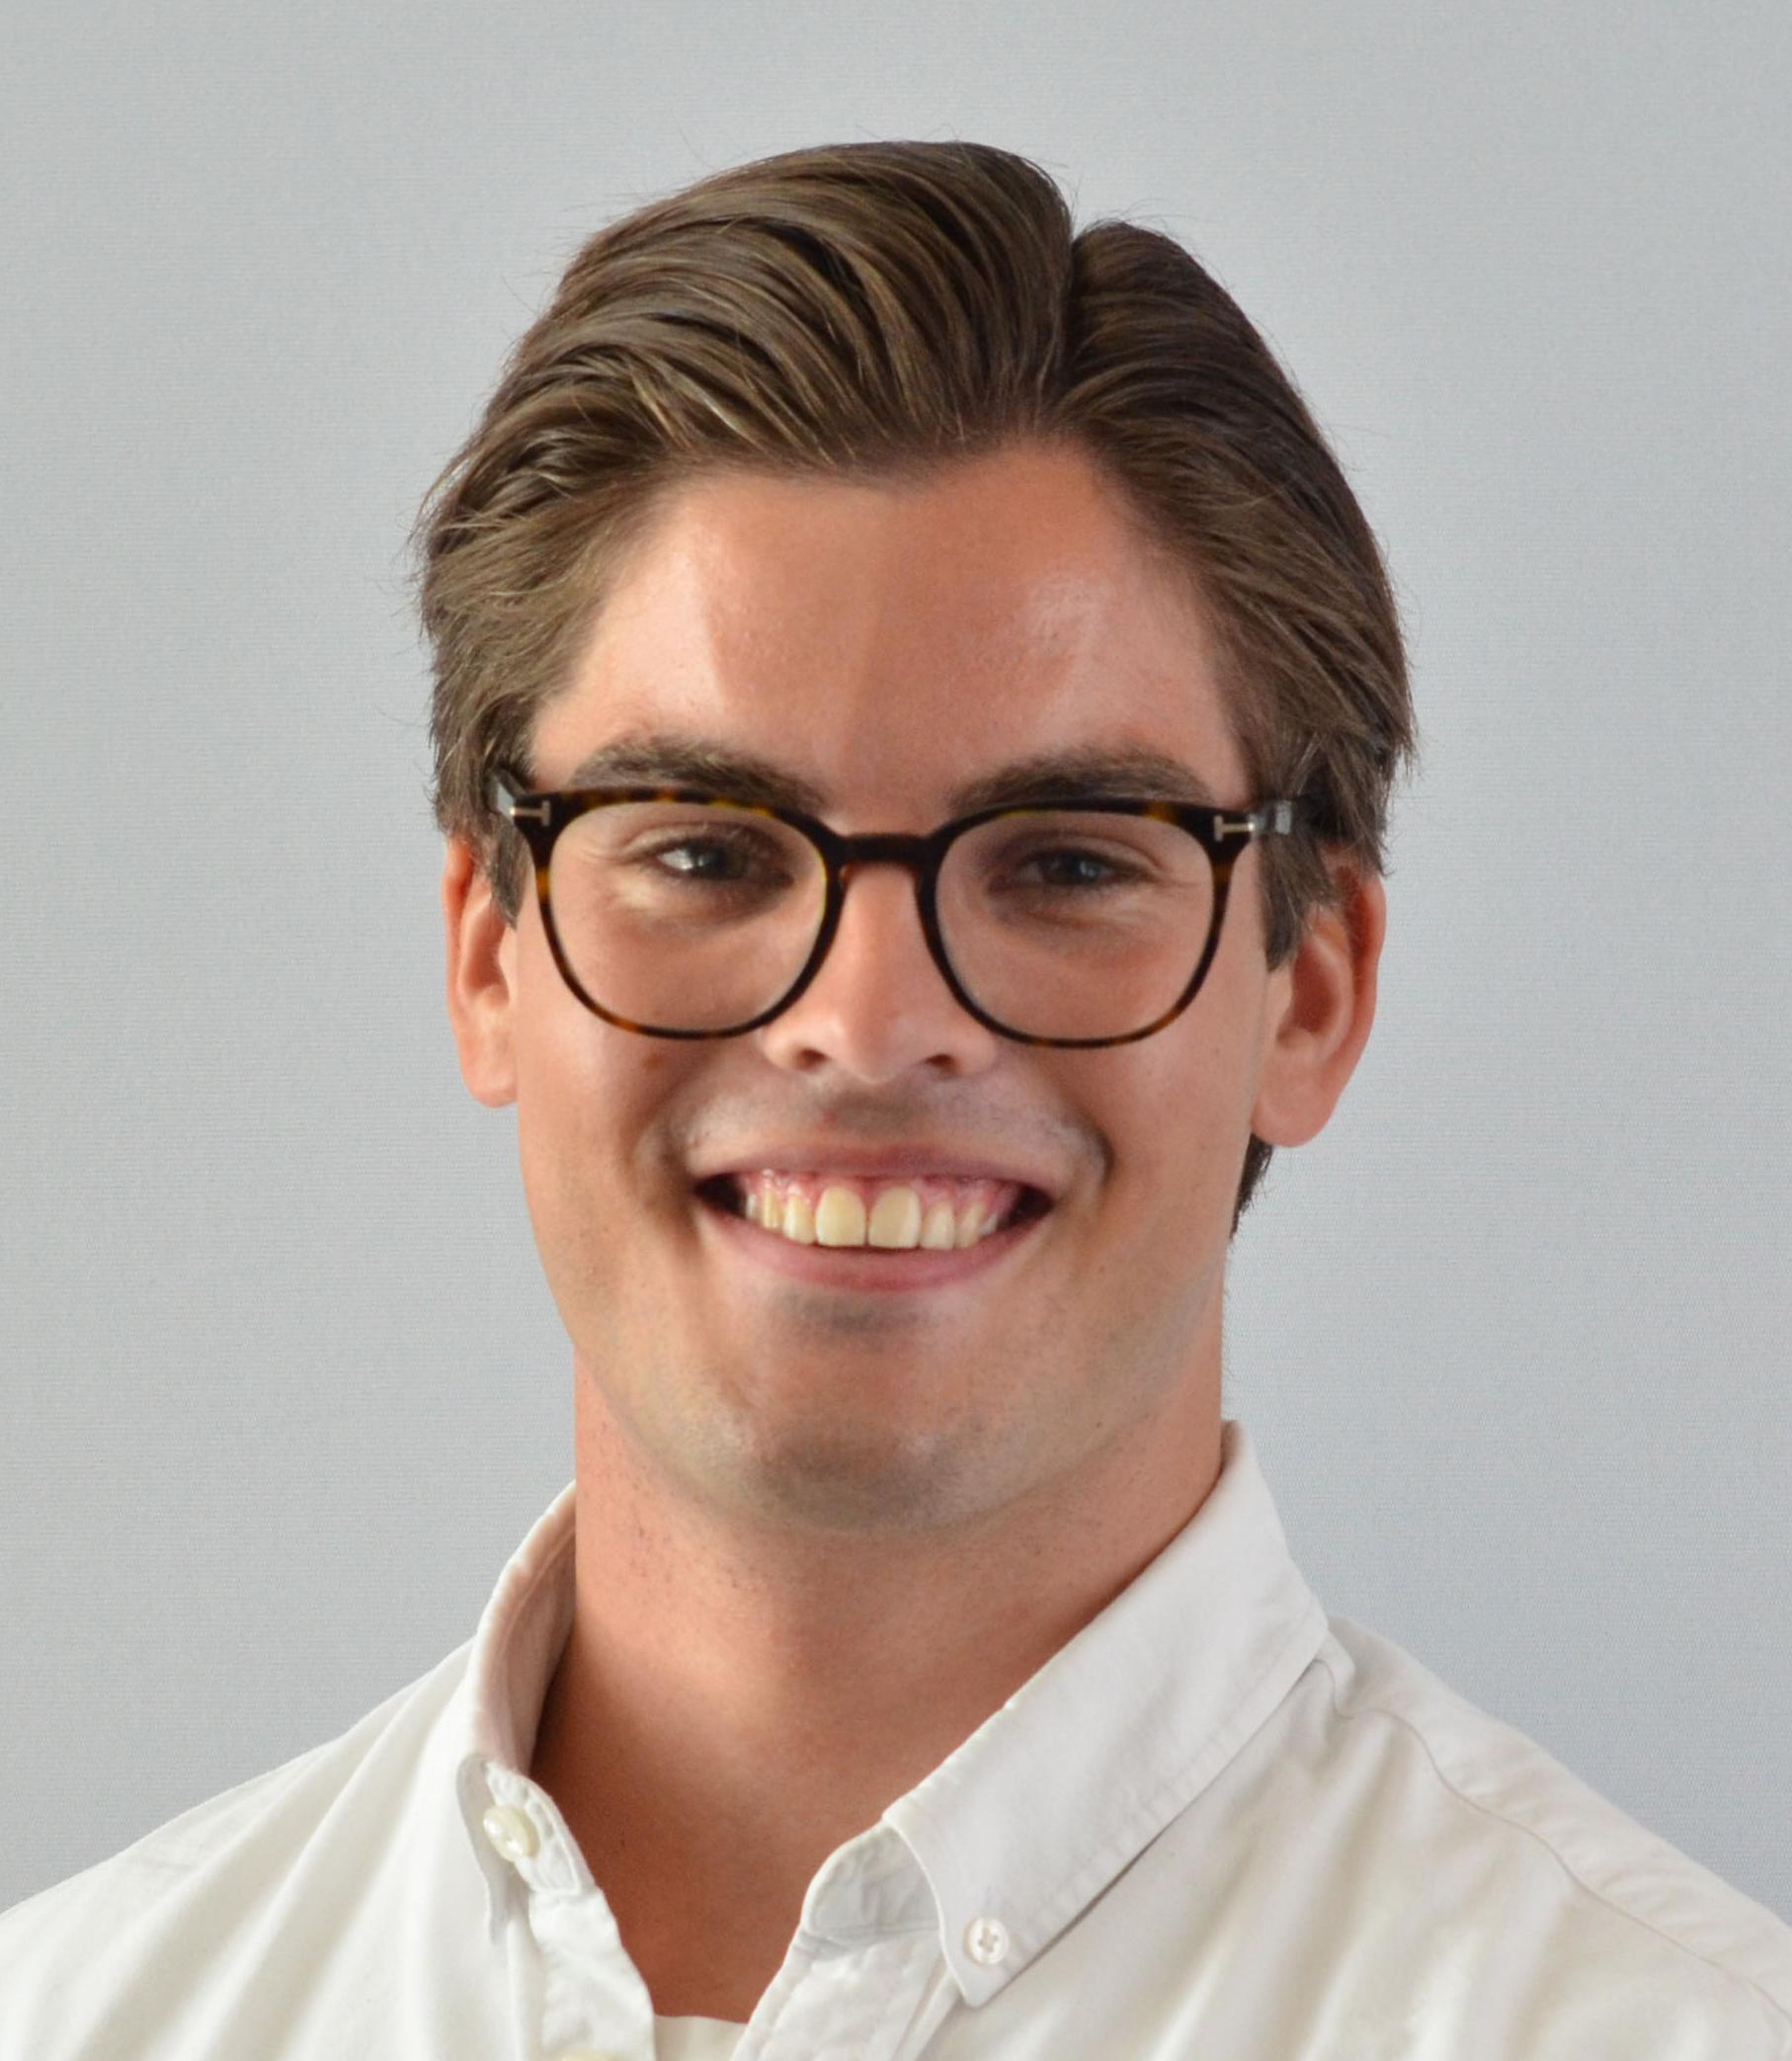
\includegraphics[width=3.5cm]{profile.jpeg}
\end{minipage}

\vspace{20pt}

% Professional Summary
\section{Professional Summary}
\needspace{5\baselineskip}
Senior Full-Stack Engineer with 4+ years of experience delivering high-impact solutions for major clients in utilities and government sectors. Currently working as a consultant at Computas AS, leading architecture and hands-on development of identity platforms, event-driven microservices, and secure data-sharing tools. Proven track record as Tech Lead for mission-critical authentication systems and modernization of legacy applications. Passionate about knowledge sharing and community building as leader of Computas' AI \& Data professional network. Holds an M.Sc. in Computer Science with focus on security.

\vspace{10pt}

% Key Competencies
\section{Key Competencies}
\needspace{6\baselineskip}
\begin{itemize}[itemsep=0.5em, leftmargin=*]
\item \cvitem{Backend Development}{.NET (C\#), Java, Kotlin, Go, Python}
\item \cvitem{Cloud \& DevOps}{Kubernetes, Docker, Azure (AKS), GCP, Terraform, Vault}
\item \cvitem{Identity \& Security}{OAuth2, OIDC, Passkeys, BankID/ID-porten integration}
\item \cvitem{Architecture}{Event-driven microservices, RESTful APIs, Kafka}
\item \cvitem{Frontend}{React, Angular, Vue.js, Next.js}
\item \cvitem{Data \& AI}{Machine learning, TensorFlow, Elasticsearch}
\end{itemize}

\vspace{10pt}
\clearpage
% Professional Experience
\section{Professional Experience}
\needspace{6\baselineskip}

\subsection{Computas AS — Senior Full-Stack Engineer / Consultant}
\textcolor{gray}{August 2021 – Present}\\
Delivering software solutions to external clients across various industries.

\vspace{10pt}
\textbf{Key Client Projects:}
\vspace{10pt}

\cventry{Elvia – ElvID Identity Platform}{Nov 2023 – Present}{Tech Lead \& Lead Developer}{}{
\needspace{10\baselineskip}
ElvID is Elvia's centralized identity platform providing single sign-on for electricity customers, internal staff, and machine-to-machine integrations. Built on Duende IdentityServer 4 and running on AKS.
\begin{itemize}[itemsep=0.3em, leftmargin=*]
\item Leading overall development, operations, and technical architecture as primary developer
\item Migrated authentication from Signicat to ID-porten
\item Implemented FREG (Norwegian National Registry) lookup for customer data
\item Introduced Passkey support for phishing-resistant biometric authentication
\item Established new integration with Maskinporten for authentication against public services
\end{itemize}
\textcolor{gray}{\textit{Tech Stack: .NET 6, Duende IdentityServer, AKS, Azure SQL, Terraform, Vault, Grafana, Kafka}}
}

\vspace{10pt}
\cventry{Elvia – OneTime Secret Sharing Service}{Mar 2025 – Present}{Developer}{}{
\needspace{5\baselineskip}
Internal secure encryption tool based on Yopass for sharing text and attachments via email and SMS.
\begin{itemize}[itemsep=0.3em, leftmargin=*]
\item Refactored and rewrote entire codebase for improved structure and testability
\item Implemented support for sharing encrypted secrets via SMS and email integration
\item Added Cloudmersive virus scanning for file attachments
\item Optimized Redis eviction policies
\end{itemize}
\textcolor{gray}{\textit{Tech Stack: Go, Vue 3, Redis, Docker, Kubernetes}}
}

\vspace{10pt}
\cventry{Elvia – Unified Messaging Platform (Convey)}{Dec 2023 – Present}{Developer}{}{
\needspace{5\baselineskip}
Central messaging service ensuring unified communication across all systems, replacing legacy Salesforce platform.
\begin{itemize}[itemsep=0.3em, leftmargin=*]
\item Developed email service with SendGrid integration
\item Co-designed service mesh and observability strategy in AKS
\item Built on .NET microservice architecture with Kafka queue technology
\end{itemize}
\textcolor{gray}{\textit{Tech Stack: ASP.NET Core, Kafka, AKS, Docker, Terraform, Vault, REST APIs, SendGrid}}
}

\vspace{15pt}
\cventry{Norwegian Police IT – UTSYS}{Sep 2021 – Oct 2023}{Functional Architect \& Full-Stack Developer}{}{
\needspace{10\baselineskip}
Modernization of Police Immigration Service's core case-processing system, migrating from monolithic to microservices.
\begin{itemize}[itemsep=0.3em, leftmargin=*]
\item Designed target architecture and migration roadmap for legacy system modernization
\item Developed document storage API with Elasticsearch full-text search
\item Implemented HashiCorp Vault for secure secrets management
\item Set up GitLab CI/CD pipelines and Docker-based development environment
\end{itemize}
\textcolor{gray}{\textit{Tech Stack: C\#, .NET 6, SQL Server, Elasticsearch, Kubernetes, Docker, Vault, Angular, GitLab}}
}

\subsection{Norconsult AS — System Consultant / Project Manager \\ (Part-time/Summer intern)}
\textcolor{gray}{February 2017 – February 2020}
\begin{itemize}[itemsep=0.3em, leftmargin=*]
\item Workday HR Implementation (2017-2019): Led enterprise-wide HR system migration
\item CV Generation Tool (2019): Project manager for automated CV system integrated with Workday
\item Developed VBA automation scripts and API design for personnel data retrieval
\end{itemize}

\vspace{10pt}

\subsection{Gi Gaven Videre, gigavenvidere.no (Pro-bono)}
\textcolor{gray}{2023}
\begin{itemize}[itemsep=0.3em, leftmargin=*]
\item Assisted in creating semi-automated settlement-workflows in Google App Scripts for the charity platform  
\item Implemented support for generated Vipps QR code in their digital giftcard
\end{itemize}
\textcolor{gray}{\textit{Tech Stack: Javascript, Google Apps Script, Sanity  }}

\vspace{10pt}
% Internal Projects
\section{Internal Projects @ Computas AS}

\begin{itemize}[itemsep=0.5em, leftmargin=*]
\item \textbf{Music Jeopardy} (2023): Interactive quiz app for university recruitment \textcolor{gray}{(React, Next.js, Vercel, Pusher)}
\item \textbf{Run For Me} (2023): Charity app integrating Strava API \textcolor{gray}{(Kotlin, Spring Boot, Google Cloud Run)}
\item \textbf{HR Dashboard} (2020): Employee data visualization with ETL pipeline \textcolor{gray}{(Java, Spring Boot, Kubernetes)}
\end{itemize}

\vspace{10pt}

\clearpage
% Education
\section{Education}

\textbf{M.Sc. in Computer Science (Security)} \hfill \textcolor{gray}{2019 – 2021}\\
University of Bergen\\
Thesis: "Neural Networks for
Lossy Weakly-Private Information Retrieval" at Simula Research Laboratory. Private File Retrieval with Generative Adversarial Networks.

\vspace{10pt}

\textbf{B.Sc. in Computer Science} \hfill \textcolor{gray}{2017 – 2019}\\
University of Bergen

\vspace{10pt}

\textbf{Additional Studies}\\
\textcolor{gray}{University of Oslo - Informatics with focus on Nanotechnology (2016-2017)}\\
\textcolor{gray}{BI Norwegian Business School - Business Administration (2015-2016)}

\vspace{10pt}

% Roles & Responsibilities
\section{Roles \& Responsibilities}

\textbf{Leader, AI \& Data Professional Network} at Computas \hfill \textcolor{gray}{2024 – Present}
\begin{itemize}[itemsep=0.3em, leftmargin=*]
\item Organize monthly knowledge-sharing sessions focused on AI agents
\item Plan and facilitate workshops/talks for internal and external knowledge events
\item Drive competence development agenda for the network
\end{itemize}

\textbf{Workshop Presenter}: "AI Developer Tools" \hfill \textcolor{gray}{2023}

\vspace{10pt}

% Certifications & Training
\section{Certifications \& Training}

\begin{itemize}[itemsep=0.5em, leftmargin=*]
\item \textbf{Power BI Data Analyst} - Glasspaper (2023)\\
\textcolor{gray}{Comprehensive course covering data modeling, DAX, visualizations, and dashboard design}
\item \textbf{Agile Team Leadership} - Computas (2022)\\
\textcolor{gray}{Training in agile methodologies, team dynamics, and leadership in software development contexts}
\item \textbf{Consultancy School} - Computas (2025)\\
\textcolor{gray}{Internal program covering consulting skills, client communication, and project management}
\end{itemize}

\vspace{5pt}

% Languages
\section{Languages}
\textbf{Norwegian}: Native \quad \textbf{English}: Fluent \quad \textbf{Spanish}: Intermediate

\end{document}
